\renewcommand{\prevlecture}{4 }
\renewcommand{\thislecture}{5 }
\renewcommand{\nextlecture}{6 }

%
% Cover page
%

\title[PHYS 201 / Lecture \thislecture]
{
  PHYS 201 / Lecture \thislecture\\
  {\it Electric current / connection with magnetic phenomena;\\
        Magnetic field, Lorentz force; Cyclotron motion;\\
        Biot-Savart law and applications}\\
}

\author[C.Andreopoulos] {
  Professor Costas Andreopoulos\inst{1,2}, {\it FHEA}
}
\institute[Liverpool/STFC-RAL] {
   \inst{1} University of Liverpool, Department of Physics\\
   \vspace{0.1cm}
   \inst{2} U.K. Research \& Innovation (UKRI), Science \& Technology Facilities Council,\\
            Rutherford Appleton Laboratory, Particle Physics Department\\
   \vspace{0.5cm}
   {\it {\color{magenta} Lectures delivered at the University of Liverpool, 2020-21}}\\
   \vspace{0.2cm}
}
\date{\today}

\titlegraphic{
  
\includegraphics[height=25px]{./images/logo/liverpool.png}
  \hspace{3px}
  
\includegraphics[height=30px]{./images/logo/ral.png}
}


\begin{frame}[plain]
  \titlepage
\end{frame}

% ------------------------------------------------------------------------------
% ------------------------------------------------------------------------------

%
% Revision of previous lecture
%

\renewcommand{\lecturesummarytitle}{Revision }

\renewcommand{\summarizedlecture}{4 }

%
%
%

\begin{frame}{Lecture \summarizedlecture - \lecturesummarytitle}

\begin{itemize}

  \item With regards to electrical properties, there are 2 types of materials
   \begin{itemize}
     \item materials that conduct electricity: {\bf conductors}
     \item materials that do not conduct electricity: {\bf insulators (dielectrics)}
   \end{itemize}

   \vspace{0.2cm}

   \item A conductor is an object or type of material
         which {\bf contains electric charges that are relatively free to move}
  \begin{itemize}
     \item A {\em \bf perfect conductor} has an {\bf unlimited supply of free charges}.
     \item There are no perfect conductors, but many substances come close!
      \begin{itemize}
           \item e.g. the free charge density in copper is 1.8 $\times$ 10$^{10}$ C/$m^3$.
      \end{itemize}
   \end{itemize}

   \vspace{0.2cm}

   \item If we place a {\bf conductor within an external electric field}:
     \begin{itemize}
       \item The electric field vanishes everywhere inside a conductor.
       \item The potential is constant inside a conductor.
       \item Charge accumulates in the surface.
       \item The field on the surface of a conductor has no tangential component.
     \end{itemize}

\end{itemize}

\end{frame}

%
%
%

\begin{frame}{Lecture \summarizedlecture - \lecturesummarytitle (cont'd)}

\begin{itemize}

   \item Capacitance (C) denotes the ability of a body to store electric charge.
             For a system of two conductors, one with charge +Q held at
             potential $V_{+}$ and one with charge -Q held at potential $V_{-}$,
             the capacitance is a positive
             quantity defined as:
      \begin{equation*}
          C = \frac{Q}{V_{+} - V_{-}}
      \end{equation*}
      Its SI unit is the {\bf Farad (F)} defined as one Coulomb per Volt.

   \vspace{0.1cm}

   \item Calculating the capacitance for simple systems:

        \begin{itemize}
         {\small
              \item Use Gauss' law to calculate the electric field $\vec{E}$
                        in terms of the charge Q stored in one of the conductors:
                       $\oint_{S} \vec{E} \cdot d\vec{S} = Q/\epsilon_0$

              \item Once $\vec{E}$ is known, calculate the potential
                        difference V between the two conductors as:
                        $V := {\Delta}V = V_{+} - V_{-} = - \int_{-}^{+} \vec{E} \cdot d\vec{\ell}$

               \item From the known charge Q in the positive conductor and
                         the potential difference V between the conductors,
                         calculate $C = Q/V$
        }
        \end{itemize}

\end{itemize}

\end{frame}


%
%
%

\begin{frame}{Lecture \summarizedlecture - \lecturesummarytitle (cont'd)}

\begin{itemize}

   \item We studied a simple system: The {\bf parallel plate capacitor}

   \item The electric field between the plates was found to be:
      \begin{equation*}
        E = \frac{\sigma}{\epsilon_0}
      \end{equation*}

   \item The parallel plate capacitor has capacitance:
      \begin{equation*}
          C = \epsilon_0 \frac{A}{d}
      \end{equation*}
      It depends only on the geometrical characteristics of the capacitor.

   \item Energy stored in the parallel plate capacitor:
      \begin{equation*}
          U = \frac{Q^2}{2C} \;\;\;\; or \;\;\;\;
          U = \frac{1}{2} C V^2 \;\;\;\; or \;\;\;\;
          U = \frac{1}{2} Q V
      \end{equation*}
      and confirmed that:
      \begin{equation*}
          U = \frac{\epsilon_0}{2} \int_{all\;space} |\vec{E}(\vec{r})|^2  d\tau
      \end{equation*}

\end{itemize}

\end{frame}

%
%
%

\begin{frame}{Lecture \summarizedlecture - \lecturesummarytitle (cont'd)}

\begin{itemize}

   \item  {\bf Electric dipole}:
          Point charges +q and -q at a {\em small distance} d.\\

          \vspace{0.1cm}

   \item  An electric dipole its described by its {\bf electric dipole moment} $\vec{p} = q \vec{d}$\\
          \begin{itemize}
                 \item A vector pointing from the negative to the positive charge
           \end{itemize}

          \vspace{0.1cm}

   \item  An electric dipole creates a potential field V given by
          \begin{equation*}
            V \approx \frac{1}{4\pi\epsilon_0} \frac{\vec{p} \cdot \hat{r}}{r^2}
          \end{equation*}

   \item  An electric field $\vec{E}$ exerts to an electric dipole with moment $\vec{p}$
          a torque $\vec{T} = \vec{p} \times \vec{E}$

          \vspace{0.1cm}

   \item  Electric fields induce dipole moments in the direction of the field (or align
              towards the direction of the field polar molecules with permanent dipole moments)
              and generate macroscopic polarisation.

          \vspace{0.1cm}

   \item  The {\bf polarisation} $\vec{P}$ of a material is defined as the
          {\bf amount of electric dipole moment per unit volume}.\\

\end{itemize}

\end{frame}


%
%
%

\begin{frame}{Lecture \summarizedlecture - \lecturesummarytitle (cont'd)}

\begin{itemize}

   \item  The polarisation induces surface and volume polarisation charges.
          The corresponding densities are
          $\sigma_P = \vec{P} \cdot \hat{n}$ and $\rho_P = - \vec{\nabla} \cdot \vec{P}$

          \vspace{0.1cm}

    \item In the presence of dielectrics,  Gauss's law need to be generalised
          to include both free charges we also have induced polarisation charges:
          \begin{equation*}
             \vec{\nabla} \cdot \Big( \epsilon_0 \vec{E} + \vec{P} \Big) = \rho_f
              \;\;\;\; and \;\;\;\;
              \oint  \Big( \epsilon_0 \vec{E} + \vec{P} \Big) \cdot d\vec{S} = Q_f
          \end{equation*}
          where $\rho_f$ is the free charge density and $Q_f$ the amount of free charge.

          \vspace{0.1cm}

    \item The vector
           $\vec{D} = \epsilon_0 \vec{E} + \vec{P}$ is the electric displacement vector
          \begin{itemize}
             \item In SI, the electric displacement unit is $C/m^2$.
          \end{itemize}

          \vspace{0.1cm}

    \item For {\bf linear dielectrics},
              $\vec{P} = \chi_{e} \epsilon_0 \vec{E}$ and, therefore,
              $\vec{D} = \epsilon_r \epsilon_0 \vec{E}$,
              where
              $\chi_{e}$ is the electric susceptibility of the material and
              $\epsilon_r = 1 + \chi_e$ is the relative permittivity (dielectric constant).

 \item A dielectric with relative permittivity $\epsilon_r$ inserted
         between the plates of a parallel plate capacitor, increases
         its capacitance by a factor of $\epsilon_r$.

\end{itemize}

\end{frame}

%
%
%

\begin{frame}{Maxwell's equation we know so far}

In vacuum (static case):

\begin{center}
 {
  \begin{table}[H]
    \begin{tabular}{|l|c|c|}
      \hline
          & {\it Integral form} & {\it Differential form} \\
      \hline
      {\bf Gauss's law} &
        $\oint \vec{E} \cdot d\vec{S} = Q_{enclosed} / \epsilon_0$ &
        $\vec{\nabla} \cdot \vec{E} = \rho / \epsilon_0$ \\

      {\bf Circuital law} &
        $\oint \vec{E} \cdot d\vec{\ell} = 0$ &
        $\vec{\nabla} \times \vec{E} = 0$ \\
      \hline
    \end{tabular}
  \end{table}
 }
\end{center}

In the presence of materials (static case):

\begin{center}
 {
  \begin{table}[H]
    \begin{tabular}{|l|c|c|}
      \hline
          & {\it Integral form} & {\it Differential form} \\
      \hline
      {\bf Gauss's law} &
        $\oint \vec{D} d\vec{S} = Q_{enclosed; free}$ &
        $\vec{\nabla} \cdot \vec{D} = \rho_{free}$ \\

      {\bf Circuital law} &
        $\oint \vec{E} d\vec{\ell} = 0$ &
        $\vec{\nabla} \times \vec{E} = 0$ \\
      \hline
    \end{tabular}
  \end{table}
 }
\end{center}

\end{frame}


%
% Plan for this lecture
%

\begin{frame}{Plan for Lecture \thislecture}

\begin{itemize}
   \item Electric current
      \begin{itemize}
           \item The {\em microscopic} view
      \end{itemize}
   \item Magnetic phenomena
      \begin{itemize}
           \item Connection with the electric current
      \end{itemize}
   \item The magnetic field
   \item Magnetic force on a charge
      \begin{itemize}
           \item Cyclotron motion and cyclotrons
      \end{itemize}
   \item Magnetic force on a current
   \item Magnetic forces do no work
   \item Calculating magnetic fields: The Biot-Savart law
     \begin{itemize}
           \item Magnetic field around a straight wire
      \end{itemize}
\end{itemize}

\end{frame}

% ------------------------------------------------------------------------------
% ------------------------------------------------------------------------------

%
%
%

\begin{frame}{Electric current}

An {\bf electric current is a flow of electric charge.}\\
\vspace{0.2cm}
It is represented by the amount of charge passing through per unit time.
\begin{equation*}
  I = \frac{dQ}{dt}
\end{equation*}

In SI, the unit of the electric current is the {\bf Ampere (A)}.
One Ampere is a charge change of 1 C over a period of 1 s.
\begin{itemize}
{\scriptsize
   \item Actually, this is how we define the Coulomb!
             We will see the actual definition of the Ampere once we have studied the magnetic force
              between two parallel conductors.\\
}
\end{itemize}

\vspace{0.1cm}

\begin{columns}
  \begin{column}{0.45\textwidth}
   \begin{center}
    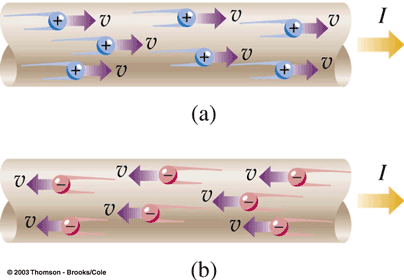
\includegraphics[width=0.78\textwidth]{./images/schematics/current_direction_convention.png}
   \end{center}
  \end{column}
  \begin{column}{0.55\textwidth}
     Note that, {\em by convention}, the current direction is {\bf the direction of flow of positive charges}.
  \end{column}
\end{columns}

\end{frame}

%
%
%

\begin{frame}{Electric current: The {\em microscopic} view }

Consider a ``tube'' within a conducting material:\\
\vspace{0.2cm}

\begin{columns}
  \begin{column}{0.67\textwidth}
    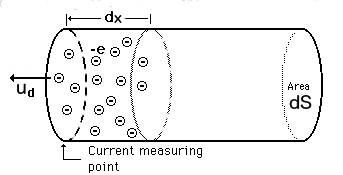
\includegraphics[width=0.98\textwidth]{./images/schematics/current_microscopic_view.png}
  \end{column}
  \begin{column}{0.33\textwidth}
      Let
      \begin{itemize}
           \item n be the carrier density,
           \item q be the charge of each carrier, and
           \item $\vec{u}_{d}$ be the average carrier velocity
      \end{itemize}
  \end{column}
\end{columns}

\vspace{0.4cm}

The amount of charge passing through a cross-section of area dS is:
\begin{equation*}
  dQ = n q d\vec{x} \cdot d\vec{S}
        = n q \Big( \vec{u}_{d} dt \Big) \cdot d\vec{S}
\end{equation*}

\end{frame}


%
%
%

\begin{frame}{Electric current: The {\em microscopic} view }

Therefore, the current I through the area dS is given by:
\begin{equation*}
  I = \frac{dQ}{dt} = \frac{n q \Big( \vec{u}_{d} dt \Big)
    d\vec{S}}{dt} = n q \vec{u}_{d} \cdot d\vec{S}
\end{equation*}

The total amount of current flowing through the entire surface S
is given by integrating the above result over S:
\begin{equation*}
  I = \int_{S} n q \vec{u}_{d} \cdot d\vec{S}
\end{equation*}

We can define a {\bf current density} $\vec{j}$ as follows:
\begin{equation*}
  I = \int_{S} \vec{j} \cdot d\vec{S}
\end{equation*}
The  current density is the {\bf current per unit area  of cross-section}.\\

You can easily see from the above that:
\begin{equation*}
  \vec{j} = n q \vec{u}_{d}
\end{equation*}

\end{frame}

%
%
%

\begin{frame}{Electric current: The {\em microscopic} view }

In general
\begin{equation*}
  \vec{j} = \sigma \vec{E}
\end{equation*}
where $\sigma$ is the {\bf conductivity} of the material.
It is an intrinsic property of a material and
 a {\bf measure of its ability to conduct an electric current.}
\begin{itemize}
   \item for a perfect insulator: $\sigma$=0, whereas
             for a perfect conductor: $\sigma$=$\infty$
\end{itemize}
In SI, the unit of conductivity is $1/(\Omega \cdot m)$ (= $S/m$).\\

\vspace{0.2cm}

The inverse of conductivity is called, {\bf resistivity} ($\rho$):
\begin{equation*}
  \rho = \frac{1}{\sigma}
\end{equation*}

Typical values:\\
\begin{center}
{\scriptsize
    \begin{table}
    \begin{tabular}{|c|c|c|}
      \hline
        Material &
        $\rho$  $(\Omega \cdot m)$ at $20^{o}$C &
        $\sigma$  $({\Omega}^{-1} \cdot m^{-1})$ at $20^{o}$C \\
      \hline
        Graphene &  1.00$\times$10$^{-8}$ & 1.00$\times$10$^{8}$ \\
        Copper   &  1.68$\times$10$^{-8}$ & 5.96$\times$10$^{7}$ \\
        Glass    &  10$^{11}$-10$^{15}$ & 10$^{-15}$-10$^{-11}$ \\
      \hline
    \end{tabular}
    \end{table}
}
\end{center}

\end{frame}

%
%
%

\begin{frame}{Electric current: The {\em microscopic} view }

Assume that a current I is {\bf flowing out of a volume $\tau$}
through its surrounding closed surface S.
The current flowing through the surface S is given by the negative (*)
rate of change of the charge contained in the volume $\tau$:
\begin{equation*}
   I = - \frac{dQ}{dt}
\end{equation*}
where Q is the volume integral of the charge density $\rho$:
\begin{equation*}
   Q = \int_{\tau} \rho d\tau
\end{equation*}
Therefore
\begin{equation*}
   I = - \frac{d}{dt} \int_{\tau} \rho d\tau = - \int_{\tau} \frac{d\rho}{dt} d\tau
\end{equation*}
\begin{equation*}
   I = \oint_{S} \vec{j} \cdot d\vec{S}
     \xRightarrow{\oint_{S} \vec{F} \cdot d\vec{S} = \int_{\tau} \vec{\nabla} \cdot \vec{F} d\tau}
   I = \int_{\tau} \vec{\nabla} \cdot \vec{j} d\tau
\end{equation*}

\noindent\rule{2cm}{0.4pt}\\
{\scriptsize
 (*) Current flows out, so the amount of charge in {\bf decreases}.\\
}

\end{frame}

%
%
%

\begin{frame}{Electric current: The {\em microscopic} view }

Equating the right-hand sides of the previous two equations, we have:
\begin{equation*}
  \int_{\tau} \vec{\nabla} \cdot \vec{j} d\tau = - \int_{\tau} \frac{d\rho}{dt} d\tau \Rightarrow
  \int_{\tau} \Big( \vec{\nabla} \cdot \vec{j} +\frac{d\rho}{dt} \Big) d\tau = 0
\end{equation*}

\begin{equation*}
    \vec{\nabla} \cdot \vec{j} +\frac{d\rho}{dt} = 0
\end{equation*}

\vspace{0.2cm}

The divergence of the current density is zero except for points where the
net charge is introduced to or removed from the system.\\

\vspace{0.2cm}

This result is known as the {\bf continuity equation}.\\

\vspace{0.2cm}

{\bf Charge conservation leads to current conservation.}\\

\end{frame}


%
% Worked example
%

{
\setbeamercolor {frametitle} {bg=eBG1}
\setbeamercolor {author in head/foot} {bg=eBG1}
\setbeamercolor {title in head/foot} {bg=eBG2}
\setbeamercolor {date in head/foot} {bg=eBG3}
\setbeamercolor {date in head/foot} {fg=eFG3}

%
%
%

\begin{frame}{Worked example}

\begin{blockexmplque}{Question}
Near Earth, the density of protons in the solar wind (a stream of particles from the Sun)
is 8.70 $cm^{-3}$, and their speed is 470 km/s.
\begin{itemize}
 \item Find the current density of these protons.
 \item If the Earth magnetic field did not deflect the protons, what total current would Earth
           receive?
\end{itemize}
The radius of the Earth is 6.37 $\times$ 10$^6$ m.
\end{blockexmplque}
\vspace{0.4cm}

The magnitude of the current density vector $\vec{j}$ is:
\begin{equation*}
    |\vec{j}| = n q |\vec{u}| \Rightarrow
\end{equation*}
\begin{equation*}
    |\vec{j}| =
     \Big( \frac{8.70}{10^{-6} \; m^3} \Big)
     \Big( 1.60 \times 10^{-19}\; C \Big)
     \Big( 470 \times 10^{3} \; m/s \Big) = 6.54 \times 10^{-7} A/m^2
\end{equation*}

\end{frame}

%
%
%

\begin{frame}{Worked example}

Although the total surface area of Earth is $4\pi R_{Earth}^2$ (that of a sphere), the area to be used
in a computation of how many protons in an approximately unidirectional beam (the solar wind)
will be captured by Earth is its projected area. In other words, for the beam, the encounter is with
a ``target'' of circular area $\pi R_{Earth}^2$ . \\
\vspace{0.3cm}

The rate of charge transport implied by the influx of protons is:
\begin{equation*}
    I = \Big( \pi R_{Earth}^2 \Big) |\vec{j}| \Rightarrow
\end{equation*}
\begin{equation*}
    I = \pi \Big( 6.37 \times 10^{6}\; m \Big)^2
               \Big( 6.54 \times 10^{-7}\; A/m^2 \Big) = 8.34 \times 10^{7} A
\end{equation*}


\end{frame}


} % Worked example



%
%
%

\begin{frame}{Magnetic phenomena}

As we have seen,
magnetic phenomena (as well as electric ones), were known from the antiquity. \\
\vspace{0.3cm}

\begin{columns}
  \begin{column}{0.50\textwidth}
    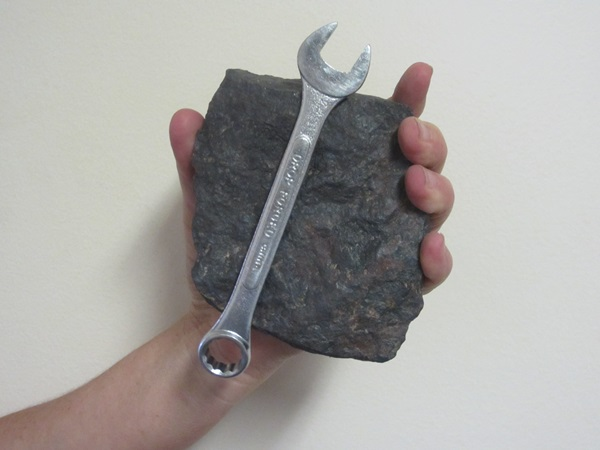
\includegraphics[width=0.99\textwidth]{./images/photos/lodestone_1.jpg}
  \end{column}
  \begin{column}{0.50\textwidth}
     {\bf Lodestones} (naturally magnetised pieces of the mineral {\em magnetite}, first found in Magnesia, Asia Minor)
     were known to be {\bf attracted to iron and other lodestones}.\\
     \vspace{0.3cm}
     Early application: The {\bf magnetic compass} (12th century AD).\\
  \end{column}
\end{columns}

\vspace{0.3cm}
{\bf Magnetic phenomena, were seemingly unrelated to electric ones}.\\

\end{frame}


%
%
%

\begin{frame}{Magnetic phenomena and electric current}

A {\bf compass is deflected in the presence of a current}
(but not in presence of stationary charges):
 {\bf A current generates a magnetic field!}\\

\begin{columns}
  \begin{column}{0.40\textwidth}
    \begin{center}
      {\small
        First observed by Oersted\\ in the early 1800's.\\
       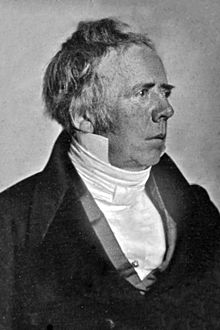
\includegraphics[width=0.60\textwidth]{./images/people/orsted.jpg}\\
        Hans Christian Oersted\\ (1777-1851)\\Danish physicist\\
      }
    \end{center}
  \end{column}
  \begin{column}{0.60\textwidth}
    \begin{center}
      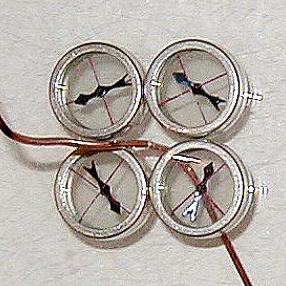
\includegraphics[width=0.85\textwidth]{./images/photos/compass_deflection_wire_current_up.jpg}\\
    \end{center}
  \end{column}
\end{columns}

\end{frame}

%
%
%

\begin{frame}{Magnetic phenomena and electric current}

{\bf A current generates a magnetic field!}\\

\begin{columns}
  \begin{column}{0.50\textwidth}
    \begin{center}
      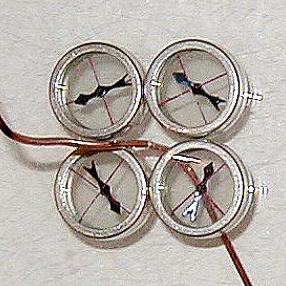
\includegraphics[width=0.90\textwidth]{./images/photos/compass_deflection_wire_current_up.jpg}\\
    \end{center}
  \end{column}
  \begin{column}{0.50\textwidth}
    \begin{center}
      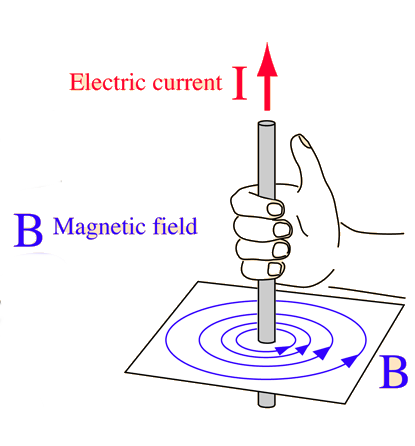
\includegraphics[width=0.90\textwidth]{./images/schematics/magnetic_field_around_wire_01.png}\\
    \end{center}
  \end{column}
\end{columns}

\vspace{0.1cm}
Interestingly, the field doesn't point towards to (or away from) the wire:\\
{\bf It circles around it}. {\it (We will calculate this field later in this lecture.)}\\

\end{frame}


%
%
%

\begin{frame}{Magnetic phenomena and electric current}

Not only a compass would be deflected in the presence of a current,
but the opposite seems to be happening as well:\\
\vspace{0.3cm}
{\bf The motion of a magnet near a conducting loop induces a current in the loop}
(but there is no current if the magnet is stationary)!

\begin{center}
 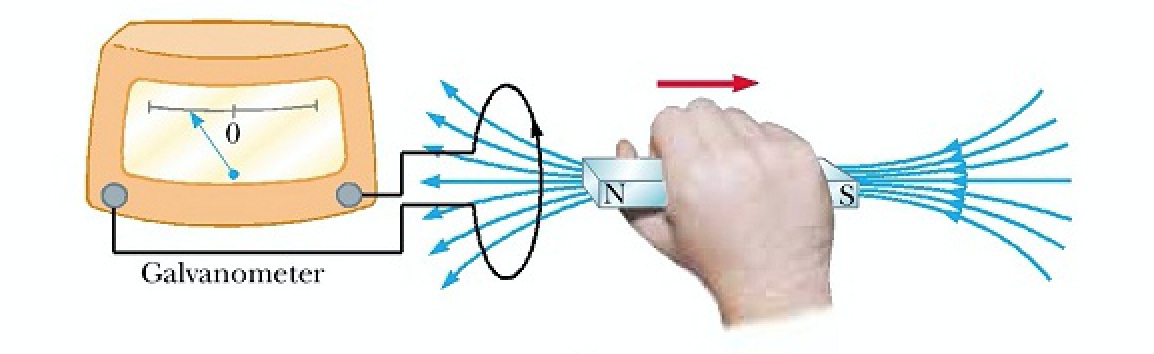
\includegraphics[width=0.99\textwidth]{./images/schematics/magnetic_field_induces_current_in_conducting_loop.png}
\end{center}

\end{frame}

%
%
%

\begin{frame}{Magnetic phenomena and electric current}

As result of the fact that a current generates a magnetic field,
{\bf a magnetic force is exerted between two wires!}\\

\begin{columns}
  \begin{column}{0.60\textwidth}
    \begin{center}
      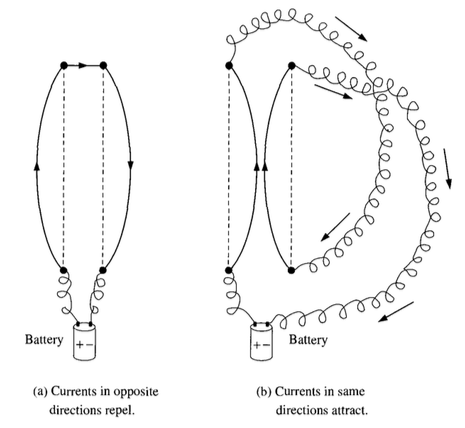
\includegraphics[width=0.90\textwidth]{./images/schematics/magnetic_force_between_wires_01.png}\\
    \end{center}
  \end{column}
  \begin{column}{0.30\textwidth}
    \begin{center}
      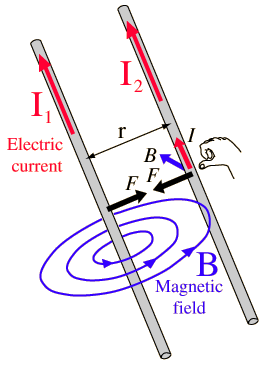
\includegraphics[width=0.90\textwidth]{./images/schematics/magnetic_force_between_wires.png}\\
      \vspace{0.2cm}
      {\small \it (We will calculate this force later in this lecture series.)}\\
    \end{center}
  \end{column}
\end{columns}

\end{frame}

%
%
%

\begin{frame}{Magnetic phenomena and electric current}

Let's reflect on the astonishing early observations:

\begin{itemize}
    \item
       {\bf Moving charges (electric currents) generate magnetic fields!}
    \vspace{0.2cm}
    \item
       {\bf Moving magnetic fields generate electric currents!}
    \vspace{0.2cm}
    \item
       {\bf There are magnetic forces between electric currents!}
    \vspace{0.2cm}
\end{itemize}

\vspace{0.4cm}

Contrary to earlier beliefs, {\bf magnetic and electric phenomena
have a common origin: the electric charge!}\\

\vspace{0.2cm}

They are not different phenomena, but {\bf different manifestations of a
single interaction!}\\

\end{frame}


%
%
%

\begin{frame}{The magnetic field}

The {\bf magnetic field is the magnetic effect of electric currents and magnetic materials}.
\begin{itemize}
   \item It is a {\bf vector field}: It permeates all space and associates a vector with each point.
\end{itemize}

\vspace{0.2cm}

In SI, the unit of the magnetic field is the {\bf Tesla (T)}.
\begin{itemize}
  \item Named in honour of Nikola Tesla (1856-1943), a
            Serbian-American physicist, engineer and inventor.
   \item The Tesla is a derived unit
       \begin{itemize}
            \item A charge of 1 C with a velocity of 1 m/s perpendicular to a
                     magnetic field of 1 T, experiences a magnetic force of 1 N ($T = N \cdot s \cdot C^{-1} \cdot m^{-1}$)\\
            \item Other common (equivalent) definitions:
                      $T = V \cdot s \cdot m^{-2} = N \cdot A \cdot m^{-1} = J \cdot A \cdot m^{-2} = Wb \cdot m^{-2}$
       \end{itemize}
   \item Another commonly used unit is the CGS one: the {\bf Gauss (G)}
       \begin{itemize}
             \item 1 G = $10^{-4}$ T
             \item Earth's magnetic field is around 1 G.
       \end{itemize}
\end{itemize}

\end{frame}

%
%
%

\begin{frame}{Typical magnetic fields}

\begin{columns}
  \begin{column}{0.40\textwidth}
  {
   \begin{center}
    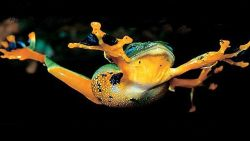
\includegraphics[width=0.88\textwidth]{./images/photos/levitating_frog_01.jpg}\\
    \vspace{0.1cm}
    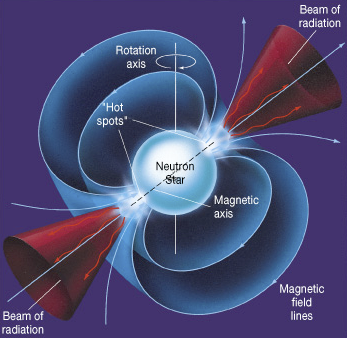
\includegraphics[width=0.88\textwidth]{./images/misc/neutron_star.png}\\
   \end{center}
  }
  \end{column}
  \begin{column}{0.60\textwidth}
   \begin{itemize}
     \item {\bf Human brain}:\\
          {\color{blue}1 pT ($10^{-12}$ T)} / {\color{magenta}10 nG = ($10^{-8}$ G)}
     \item {\bf Earth's} magnetic field:\\
          Somewhat less than {\color{blue} $10^{-4}$ T} / {\color{magenta} 1 G }
     \item {\bf Refrigerator} magnet:\\
           {\color{blue} 5 mT (5 $10^{-3}$ T)} /  {\color{magenta} 50 G}
     \item {\bf LHC} dipole magnet:\\
           {\color{blue} 10 T} / {\color{magenta} $10^{5}$ G}
     \item Field that you need to {\bf levitate a frog}:
           {\color{blue} 16 T} / {\color{magenta} 1.6 $\times$ $10^{5}$ G}
     \item {\bf Neutron stars} (magnetar):\\
            {\color{blue} 1 MT ($10^{6}$ T) - 100 GT ($10^{11}$ T)} / \\
            {\color{magenta} 10 GG ($10^{10}$ G) - 1 PG ($10^{15}$ G)}
   \end{itemize}
  \end{column}
\end{columns}

\end{frame}

%
%
%

\begin{frame}{``Magnetic charges''}

There are several similarities between electrostatics and magnetostatics:\\

\begin{columns}
  \begin{column}{0.40\textwidth}
    \begin{center}
      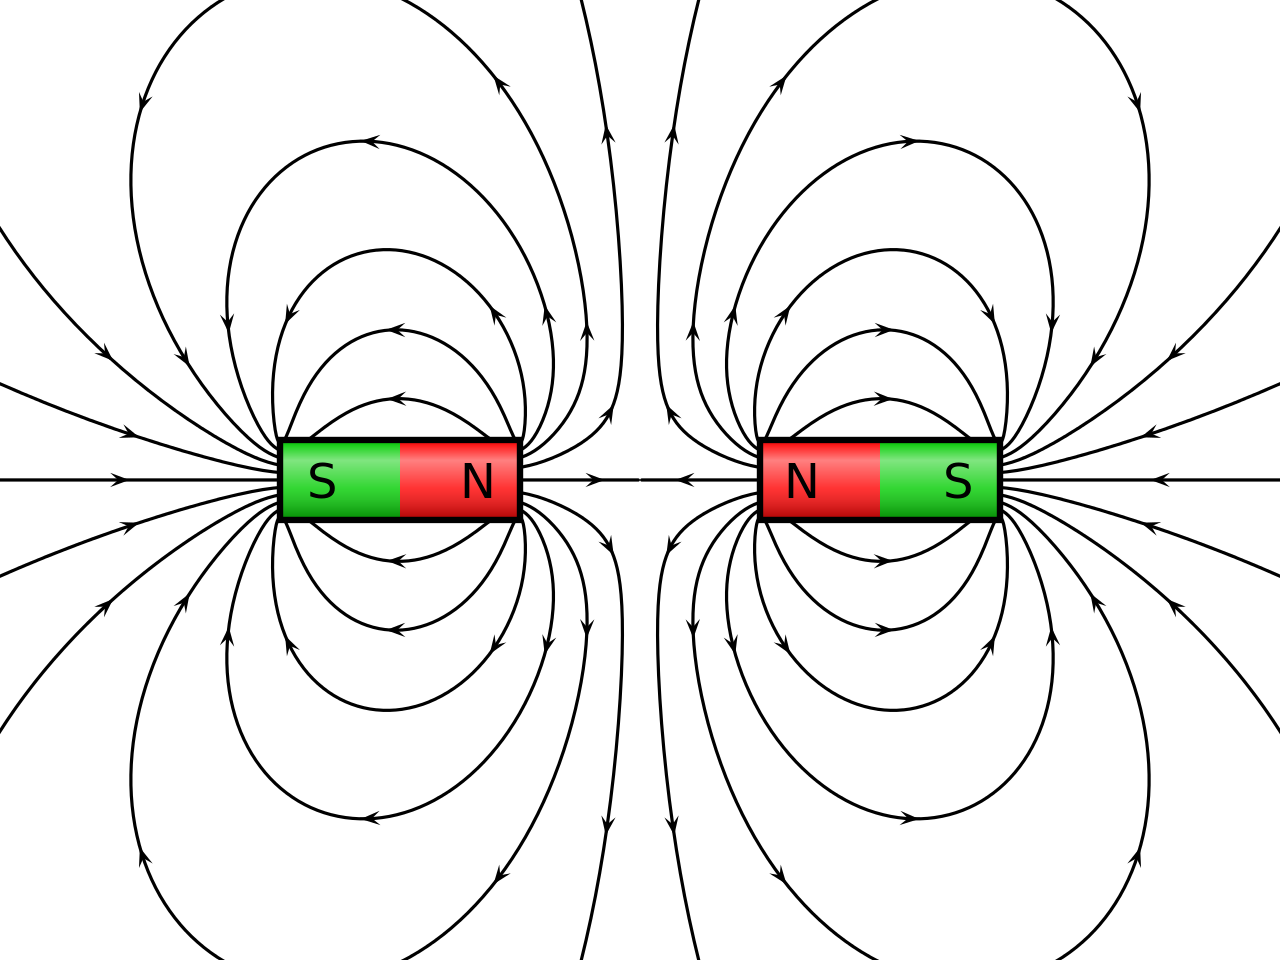
\includegraphics[width=0.90\textwidth]{./images/schematics/magnetic_field_lines_01.png}\\
    \end{center}
  \end{column}
  \begin{column}{0.60\textwidth}

\begin{itemize}
   \item We have two ``types of magnetic charges''
             (we call them {\bf North} and {\bf South} {\em poles})
   \item Same poles repel each other, while opposite poles attract each other.
   \item Magnetic field lines always start from a North pole and end in a South pole.
\end{itemize}

  \end{column}
\end{columns}

\vspace{0.3cm}

However, {\bf there is one striking difference}:
\vspace{0.1cm}
Whereas single positive or a single negative charges (electric monopoles) exist in isolation,
{\bf magnetic monopoles do not exist} (or they have not been found yet (*)).\\

\noindent\rule{2cm}{0.4pt}\\
{\scriptsize
 (*) Or, maybe we have: Google ``Blas Cabrera, Valentine's day magnetic monopole''\\
}

\end{frame}


%
%
%

\begin{frame}{Magnetic force on an electric charge}

{\bf What is the force that a magnetic field exerts on a moving charge?}\\
\vspace{0.2cm}
It was observed experimentally that the force $\vec{F}$ exerted by a magnetic field $\vec{B}$,
on a charge q moving with velocity $\vec{u}$ has a magnitude $|\vec{F}|$  that is proportional to all q,
$|\vec{u}|$ and $|\vec{B}|$:
\begin{equation*}
  |\vec{F}| \propto q |\vec{u}| |\vec{B}|
\end{equation*}

It was observed that:
\begin{itemize}
{\small
  \item magnetic force vanishes if $\vec{u}$ and $\vec{B}$ are parallel
  \item force is increasing as the angle between $\vec{u}$ and $\vec{B}$ increases
  \item the maximum force is exerted when $\vec{u}$ and $\vec{B}$ are perpendicular to each other
  \item F is not on the same plane as $\vec{u}$ and $\vec{B}$,
            but perpendicular to the plane defined by $\vec{u}$ and $\vec{B}$
}
\end{itemize}

All the above can be summarised as:
\begin{equation*}
  \vec{F} = q \vec{u} \times \vec{B}
\end{equation*}

\end{frame}

%
%
%

\begin{frame}{Magnetic force on an electric charge}

\begin{columns}
  \begin{column}{0.27\textwidth}
    \begin{center}
      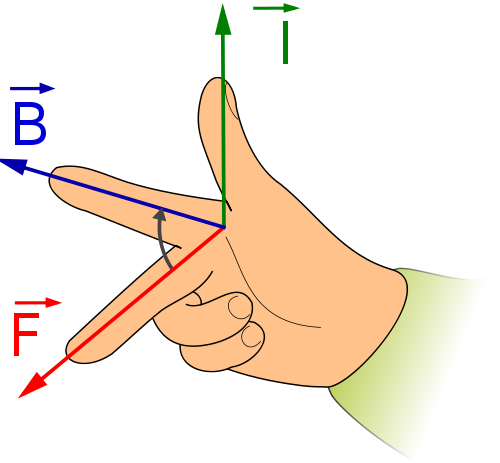
\includegraphics[width=0.90\textwidth]{./images/schematics/right_hand_rule_fbi.png}\\
    \end{center}
  \end{column}
  \begin{column}{0.73\textwidth}
      The magnetic force is given by:
      \begin{equation*}
          \vec{F} = q \vec{u} \times \vec{B}
      \end{equation*}
       Use the {\bf right-hand rule} to find the direction of $\vec{F}$.
  \end{column}
\end{columns}

\begin{columns}
  \begin{column}{0.30\textwidth}
    \begin{center}
      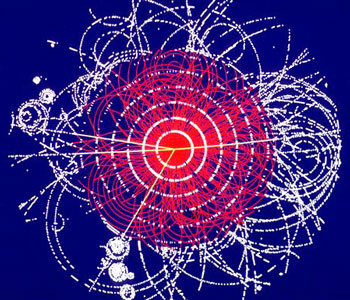
\includegraphics[width=0.99\textwidth]{./images/misc/atlas_event.jpg}\\
    \end{center}
  \end{column}
  \begin{column}{0.30\textwidth}
    \begin{center}
      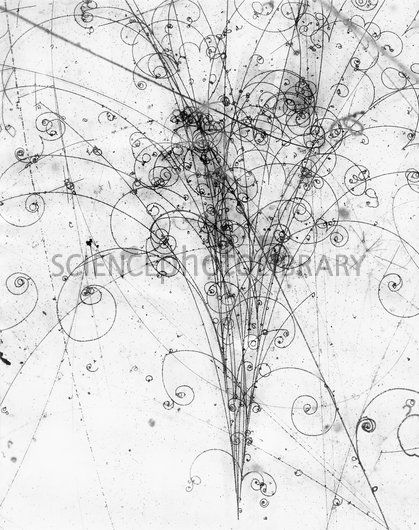
\includegraphics[width=0.70\textwidth]{./images/misc/em_particle_shower.jpg}\\
    \end{center}
  \end{column}
  \begin{column}{0.40\textwidth}
     The {\bf magnetic force} exerted on a moving charge is
     {\bf  always perpendicular to its velocity} and acts as a {\bf centripetal force}.\\
     \vspace{0.1cm}
     Charges within magnetic fields tend to {\bf follow curved trajectories}.
  \end{column}
\end{columns}

\end{frame}



%
% Worked example
%

{
\setbeamercolor {frametitle} {bg=eBG1}
\setbeamercolor {author in head/foot} {bg=eBG1}
\setbeamercolor {title in head/foot} {bg=eBG2}
\setbeamercolor {date in head/foot} {bg=eBG3}
\setbeamercolor {date in head/foot} {fg=eFG3}

%
%
%

\begin{frame}{Worked example}

\begin{blockexmplque}{Question}
A particle with charge q = -1.24 $\times 10^{-8}$ C is moving
in a magnetic field $\vec{B} = (1.4 \; T) \hat{x}$
with velocity $\vec{u} =$ $(4.19 \times 10^{4} \; m/s) \hat{x} + (-3.85 \times 10^{4} \; m/s) \hat{y}$.
Calculate in vector form the force exerted on the particle by the field.
\end{blockexmplque}
\vspace{0.4cm}

The magnetic force $\vec{F}$ exerted on the charged particle is:
\begin{equation*}
   \vec{F} = q \vec{u} \times \vec{B} \Rightarrow
\end{equation*}
\begin{equation*}
   \vec{F} = (-1.24 \times 10^{-8} C )
                  \Big\{ (4.19 \times 10^{4} \; m/s) \hat{x} + (-3.85 \times 10^{4} \; m/s) \hat{y} \Big\}
                  \times \Big\{(1.4 \; T) \hat{x} \Big\}
\end{equation*}

Notice that
$\hat{x} \times \hat{x} = 0$ and $\hat{y} \times \hat{x} = -\hat{z}$, and therefore:
\begin{equation*}
   \vec{F} = \Big(-1.24 \times 10^{-8} C \Big)
                  \Big(-3.85 \times 10^{4} \; m/s \Big)
                  \Big(1.4 \; T \Big) \Big(-\hat{z}\Big) \Rightarrow
\end{equation*}
\begin{equation*}
   \vec{F} = \Big( (-1.24)  (-3.85) 1.4 \times 10^{-4} N \Big) \Big(- \hat{z}\Big) \Rightarrow
   \vec{F} = - \Big( 6.6836 \times 10^{-4} N \Big)  \hat{z}
\end{equation*}

\end{frame}

} % Worked example

%
%
%

\begin{frame}{Lorentz force}

The total force felt by a charged body in the presence of
both electric and magnetic fields is called the {\bf Lorentz force}.

\begin{equation*}
  \vec{F} = q \Big( \vec{E} + \vec{u} \times \vec{B} \Big)
\end{equation*}

\vspace{0.3cm}

It was first derived by Oliver Heaviside or James Maxwell.
Hendrik Lorentz derived it a few years later.\\

\vspace{0.3cm}

The {\bf magnetic force is much smaller than the electric force}
unless the particle is moving at a velocity that is a significant fraction of the speed of light.

\end{frame}

%
%
%

\begin{frame}{Cyclotron motion}

Let's study the {\bf simple trajectory} of a particle moving with a
{\bf constant velocity} u in a {\bf constant magnetic field} B.\\
\vspace{0.2cm}
\begin{columns}
  \begin{column}{0.40\textwidth}
    \begin{center}
      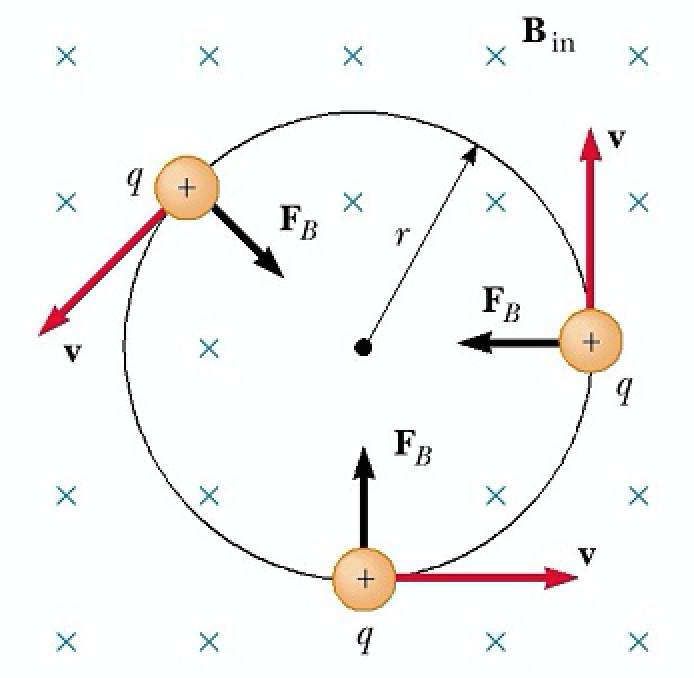
\includegraphics[width=0.90\textwidth]{./images/schematics/cyclotron_motion_01.png}\\
    \end{center}
  \end{column}
  \begin{column}{0.60\textwidth}
     Assume that a positive charge enters the magnetic field B with a velocity u
     that is perpendicular to the magnetic field which points inwards (see on the left).\\
     \vspace{0.1cm}
     The direction of the magnetic force, found using the right-hand rule,
     is also shown.
  \end{column}
\end{columns}
\vspace{0.2cm}
The magnetic force provides {\bf centripetal acceleration} and the charge will start moving
counter-clockwise, along a circle (of radius r), with a velocity that is constant in magnitude.\\

\end{frame}

%
%
%

\begin{frame}{Cyclotron motion}

The magnetic force for a charge q with velocity u perpendicular to B is:
\begin{equation*}
  F = q u B
\end{equation*}
The centripetal force (mass times centripetal acceleration) is:
\begin{equation*}
  F = m \frac{u^2}{r}
\end{equation*}
Therefore:
\begin{equation*}
  m \frac{u^2}{r} = q u B \Rightarrow
  m \frac{u}{r} = q B \Rightarrow
  m u = q B r \Rightarrow
  {\bf p = qBr}
\end{equation*}
where p is the particle momentum.
This is known as the {\bf cyclotron formula} and describes the motion of a charged particle in a cyclotron.\\
\vspace{0.2cm}
The period T (time for one revolution)
is independent of the particle velocity and it depends only on the
particle type and the magnetic field:

\begin{equation*}
  T = \frac{2\pi r}{u} \xRightarrow{m u = q B r}
  T = \frac{2\pi m}{q B}
\end{equation*}


\end{frame}


%
%
%

\begin{frame}{Cyclotron}

\begin{columns}
  \begin{column}{0.20\textwidth}
     \begin{center}
       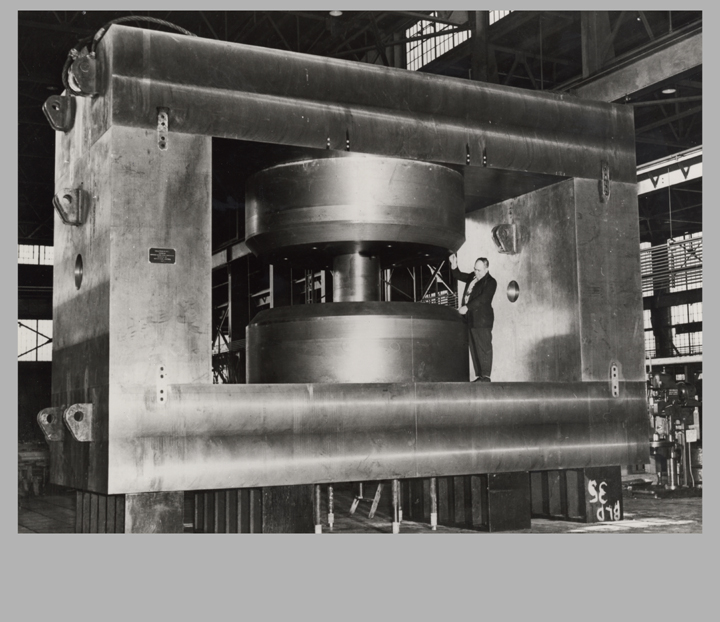
\includegraphics[width=0.99\textwidth]{./images/photos/cyclotron.jpg}\\
     \end{center}
  \end{column}
  \begin{column}{0.70\textwidth}
          {\bf A cyclotron is a type of particle accelerator}.\\
          It was invented by Ernest Lawrence in 1932 and it was the most powerful
          type of accelerator till it was superseded by the synchrotron in the 1950's.
  \end{column}
\end{columns}

\begin{center}
    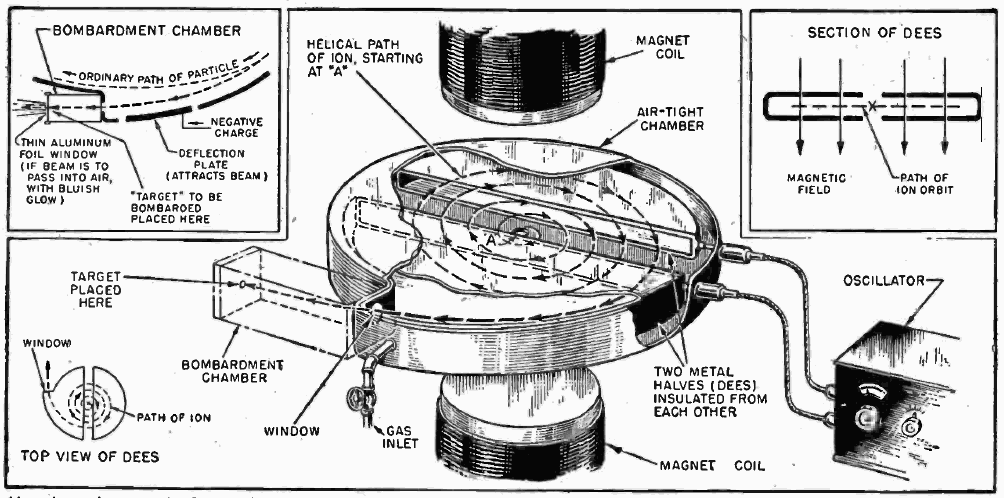
\includegraphics[width=0.85\textwidth]{./images/schematics/cyclotron_diagram.png}\\
\end{center}

\end{frame}

%
%
%

\begin{frame}{The Liverpool Cyclotron}

\begin{columns}
  \begin{column}{0.25\textwidth}
     \begin{center}
       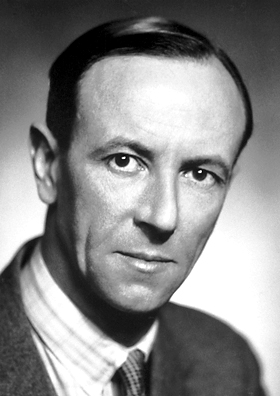
\includegraphics[width=0.80\textwidth]{./images/people/chadwick.jpg}\\
       {\scriptsize  James Chadwick\\ (1891-1974)}\\
       \vspace{0.2cm}
       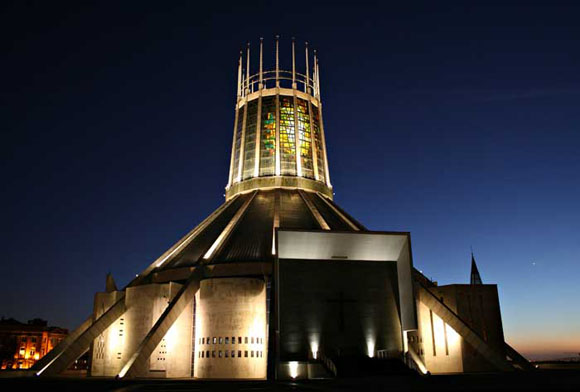
\includegraphics[width=0.80\textwidth]{./images/photos/met_cathedral.jpg}\\
       {\scriptsize  Liverpool Metropolitan Cathedral}\\
     \end{center}
  \end{column}
  \begin{column}{0.75\textwidth}
     \begin{itemize}
          \item When {\bf Chadwick} (who discovered the neutron, Nobel Prize in Physics 1935)
                    was the Head of the Physics Department at the University of Liverpool,
                    (some time before the WW2) this was the home of a very large cyclotron.
            \vspace{0.1cm}
            \begin{itemize}
                 \item You can see pieces of the D's in the VGM.
            \end{itemize}
          \vspace{0.3cm}
          \item And, in the 50's the University of Liverpool had a new synchrocyclotron, somewhere in the grounds of the
                   Metropolitan Cathedral, that was the most powerful accelerator in Europe at the time.\\
     \end{itemize}
  \end{column}
\end{columns}

\end{frame}


%
%
%

\begin{frame}{Cyclotron motion}

If the charged particle was entering the magnetic field at an angle with the field lines then it would do {\bf two motions}:\\
\vspace{0.2cm}

\begin{columns}
  \begin{column}{0.50\textwidth}
    \begin{center}
      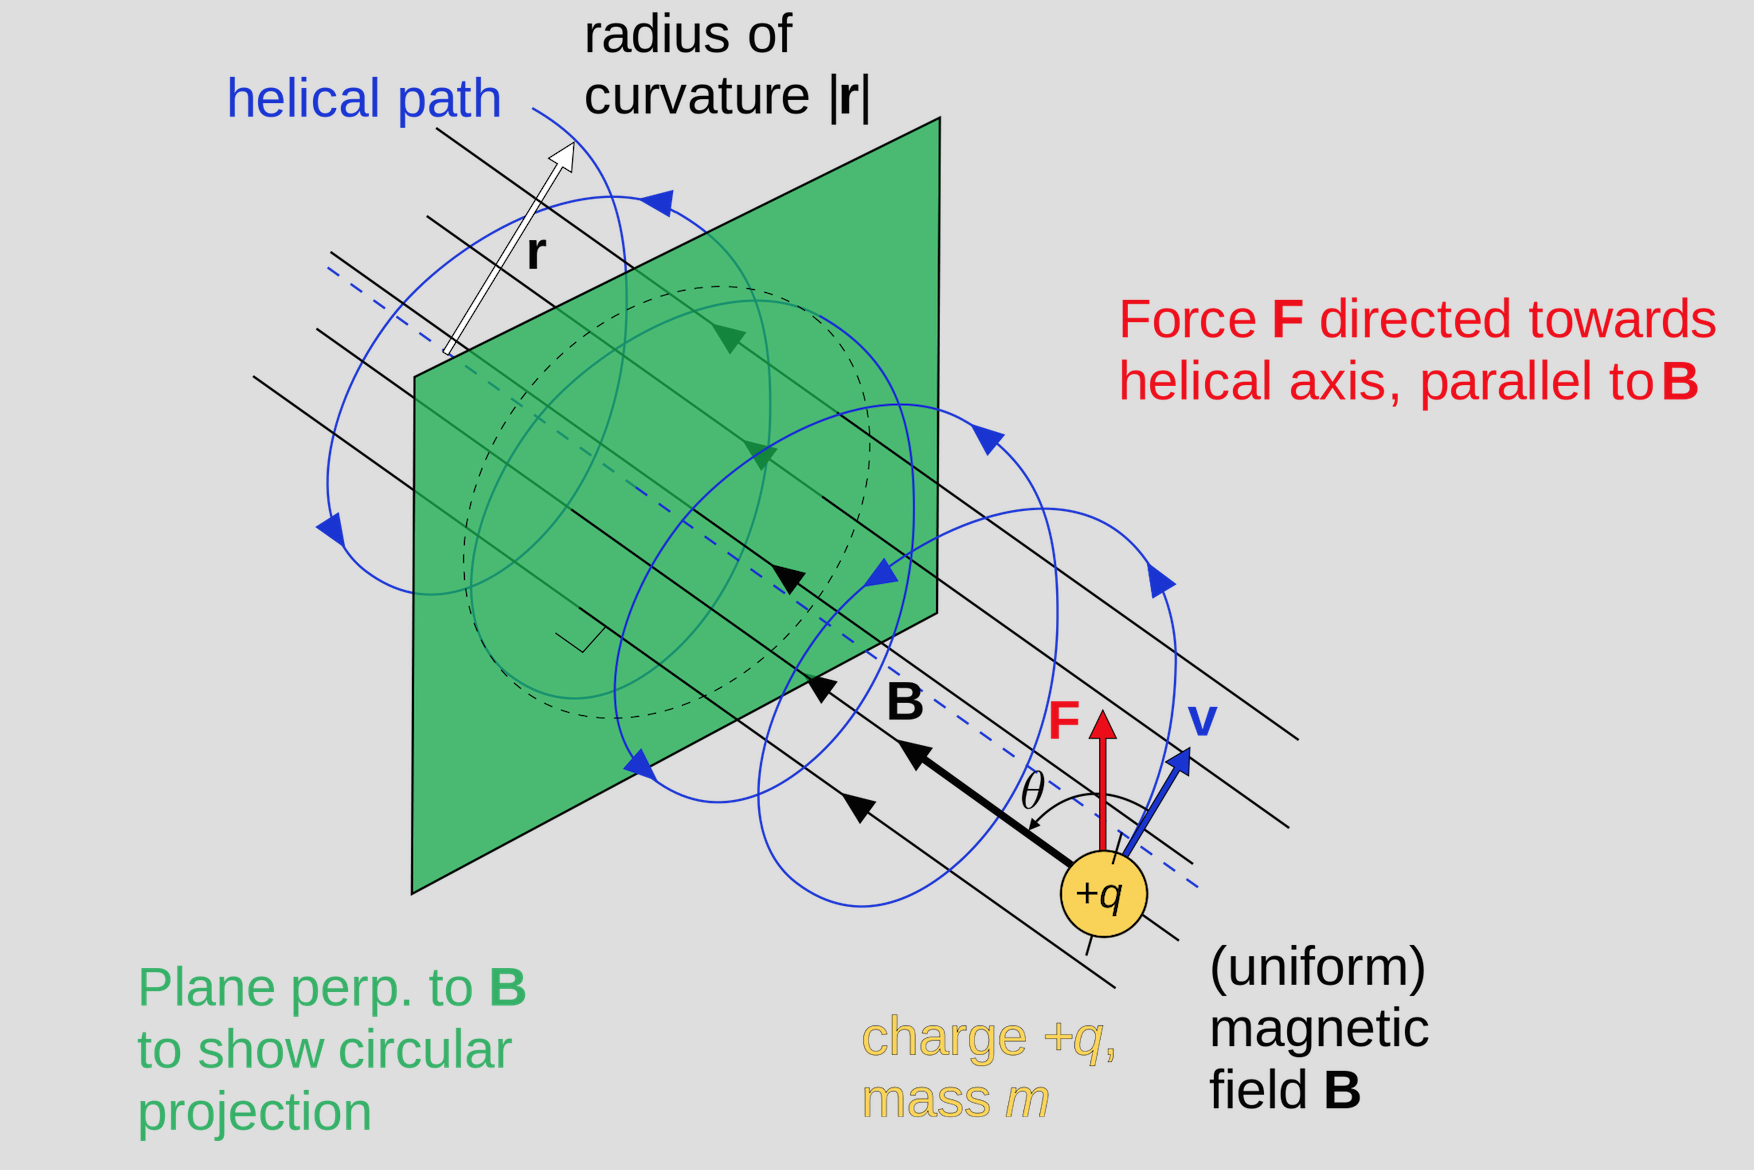
\includegraphics[width=0.99\textwidth]{./images/schematics/cyclotron_motion_02.png}\\
    \end{center}
  \end{column}
  \begin{column}{0.50\textwidth}
      \begin{itemize}
      {\small
         \item On the plane perpendicular to the field, it would move in a {\bf circular trajectory}
                   with constant velocity $u_{\perp}$ (velocity component perpendicular to the field).\\
                   Note: $F_{\perp} = q \vec{u}_{\perp} \times \vec{B} = q {u}_{\perp} B$
         \item It would also move along a {\bf straight line} in the direction of the field with constant
                   velocity $u_{\parallel}$  (component parallel to the field).\\
                   Note: $F_{\parallel} = q \vec{u}_{\parallel} \times \vec{B} = 0$
      }
      \end{itemize}
  \end{column}
\end{columns}

\vspace{0.2cm}
The combination of the two motions causes a {\bf helical trajectory}.\\

\end{frame}


%
% Worked example
%

{
\setbeamercolor {frametitle} {bg=eBG1}
\setbeamercolor {author in head/foot} {bg=eBG1}
\setbeamercolor {title in head/foot} {bg=eBG2}
\setbeamercolor {date in head/foot} {bg=eBG3}
\setbeamercolor {date in head/foot} {fg=eFG3}

%
%
%

\begin{frame}{Worked example}

\begin{blockexmplque}{Question}

\begin{columns}
  \begin{column}{0.38\textwidth}
    \begin{center}
      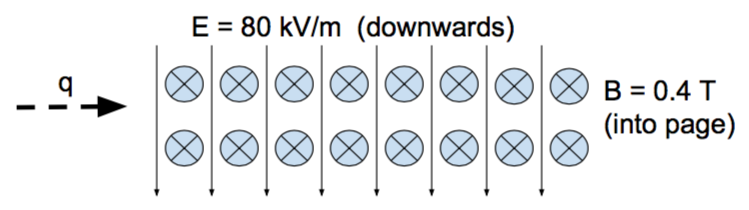
\includegraphics[width=0.98\textwidth]{./images/problems/lect4_crossed_E_B_fields.png}\\
    \end{center}
  \end{column}
  \begin{column}{0.62\textwidth}
A beam of particles with charge q enters
a region where there is a uniform electric field $\vec{E}$, of
magnitude 80 kV/m, directed downwards.
In the same region, perpendicular
  \end{column}
\end{columns}
to  $\vec{E}$ and directed into the page is a magnetic
field  $|\vec{B}|$ = 0.4T.
As the particles enter that region their
velocity is perpendicular to $\vec{E}$ and $\vec{B}$.\\
\begin{enumerate}
\item
 If the speed of the particles is properly chosen, the particles will
not be deflected by these crossed electric and magnetic fields.
What speed is selected in this case?
\item
If the electric field is cut off and the same magnetic field is maintained, the charged
particles move in the magnetic field in a circular path of radius 1.14 cm. Determine the
ratio of the electric charge to the mass of the particles.
\end{enumerate}
\end{blockexmplque}
\vspace{0.4cm}

\end{frame}

%
%
%

\begin{frame}{Worked example}

The magnetic force is: $\displaystyle   F_m = q u B $,
and the electric force is:  $\displaystyle  F_e = q E $\\
\vspace{0.2cm}

For no deflection:
\begin{equation*}
   F_m = F_e  \Rightarrow
   quB = qE  \Rightarrow
    u = \frac{E}{B} =
      \frac{80 \times 10^3 \; V/m}{0.4 \; T} = 2 \times 10^5 m/s
\end{equation*}

Once the electric field is cut off,
the particle moves in a circular path with
the magnetic force acting as the centripetal force.
\begin{equation*}
   \frac{mu^2}{r} = quB  \Rightarrow
    \frac{q}{m} = \frac{u}{Br} = \frac{E}{B^2 r}  \Rightarrow
\end{equation*}

\begin{equation*}
   \frac{q}{m} =
       \frac{80 \times 10^3 \; V/m}{\Big( 0.4 \; T\Big)^2 \Big( 1.14 \times 10^{-2} m\Big)} =
       4.38 \times 10^{7} C/kg
\end{equation*}

\end{frame}


} % Worked example



%
% Worked example
%

{
\setbeamercolor {frametitle} {bg=eBG1}
\setbeamercolor {author in head/foot} {bg=eBG1}
\setbeamercolor {title in head/foot} {bg=eBG2}
\setbeamercolor {date in head/foot} {bg=eBG3}
\setbeamercolor {date in head/foot} {fg=eFG3}

%
%
%

\begin{frame}{Worked example}

\begin{blockexmplque}{Question}
The pole pieces (the ``dees'') of a cyclotron are 50 cm in diameter, in a uniform magnetic field of 15,000 G.
\begin{enumerate}
  \item Find approximate values for the kinetic energies up to which
            (a) protons and (b) $\alpha$-particles ($He^{4}$ nuclei) could be accelerated.
  \item What oscillator frequency would be required in each case?
\end{enumerate}
The charge of the proton is $q_p = 1.6 \times 10^{-19} C$ and the mass of the proton is $m_p = 1.67 \times 10^{-27} kg$.
\end{blockexmplque}
\vspace{0.4cm}

The cyclotron formula is:
\begin{equation*}
  m u = q B r
\end{equation*}
where m is the particle mass, q its charge, u its velocity, r the radius of curvature and B the magnetic field.

\end{frame}

%
%
%

\begin{frame}{Worked example}

Hence the velocity of the particle is:
\begin{equation*}
  u = \frac{q B r}{m}
\end{equation*}

The kinetic energy of the accelerated particle is:
\begin{equation*}
  K = \frac{1}{2} m u^2 = \frac{1}{2} m \Big( \frac{q B r}{m} \Big)^2 =  \frac{q^2 B^2 r^2}{2m}
\end{equation*}

The kinetic energy K is maximal when the particle moves in a trajectory where the radius of curvature r
has the largest possible value. \\
\vspace{0.2cm}

The maximum value of r is the radius (call it R) of the dees:
\begin{equation*}
  r = R = \frac{50\;cm}{2} = 25 cm
\end{equation*}

\end{frame}

%
%
%

\begin{frame}{Worked example}

Thefore, the maximum kinetic energy for protons is given by:
\begin{equation*}
  K_{max;p}  = \frac{q_{p}^2 B^2 R^2}{2m_p}
                 = \frac{(1.6 \times 10^{-19} C)^2 (1.5T)^2 (0.25m)^2}{2(1.67 \times 10^{-27} kg)}
                     \xRightarrow{T = kg/(C s),\; J = kg \cdot m^2 / s^2}
\end{equation*}
\begin{equation*}
  K_{max;p} = 1.08 \times 10^{-12} J
\end{equation*}

An $\alpha$ particle is about 4 times heavier than a proton ($m_{\alpha} = 4 m_{p}$) and it has twice the charge ($q_{\alpha} = 2 q_{p}$).
Thefore, the maximum kinetic energy for $\alpha$'s is given by:
\begin{equation*}
  K_{max;\alpha}  = \frac{q_{\alpha}^2 B^2 R^2}{2m_{\alpha}} = \frac{\Big(2q_{p}\Big)^2 B^2 R^2}{2\Big(4m_p\Big)} =
       \frac{\cancel{4}q_{p}^2 B^2 R^2}{2 \cdot \cancel{4} m_p} = \frac{q_{p}^2 B^2 R^2}{2m_p} \Rightarrow
\end{equation*}
\begin{equation*}
  K_{max;\alpha}  =  K_{max;p}
\end{equation*}

\end{frame}

%
%
%

\begin{frame}{Worked example}

The oscillator frequency f is given by:
\begin{equation*}
  u = \Big( 2\pi f\Big) r \Rightarrow f = \frac{u}{2\pi r}
\end{equation*}
Substituting the previous expression for u ($u = q B r/m$), we have:
\begin{equation*}
 f = \frac{u}{2\pi r} = \frac{q B r }{2\pi r m} \Rightarrow
 f = \frac{q B}{2\pi m}
\end{equation*}

For protons:
\begin{equation*}
 f_{p} = \frac{q_p B}{2\pi m_p}
        = \frac{(1.6 \times 10^{-19} C)  (1.5 T)}{2\pi (1.67 \times 10^{-27} kg)}
        = \frac{1.6 \cdot 1.5}{2\pi \cdot 1.67}  \times 10^{8} \frac{C \cdot T}{kg} \xRightarrow{T = kg/(C s)}
\end{equation*}
\begin{equation*}
 f_{p} =  0.22  \times 10^{8} \frac{C}{kg}\frac{kg}{Cs} = 0.22  \times 10^{8} Hz = 22 MHz
\end{equation*}

For $\alpha$'s, the corresponding frequency is:
\begin{equation*}
 f_{\alpha} = \frac{q_{\alpha} B}{2\pi m_{\alpha}} = \frac{2q_p B}{2\pi \cdot 4m_{p}} =  \frac{1}{2}  \frac{q_p B}{2\pi m_p}  =
   \frac{1}{2} f_{p} =  \frac{1}{2}  22 MHz = 11 MHz
\end{equation*}

\end{frame}


} % Worked example



%
%
%

\begin{frame}{Magnetic force on current}

As we have seen, the force on a single moving charge q is:
\begin{equation*}
  \vec{F} = q \vec{u} \times \vec{B}
\end{equation*}

How about the {\bf force on a current} that consists of several moving charges?

\begin{equation*}
  q ...  \rightarrow \int_{V} \rho ... d\tau
\end{equation*}

\begin{equation*}
  \vec{F} = q \vec{u} \times \vec{B} \rightarrow \int_{\tau} \rho \vec{u} \times \vec{B} d\tau
                 \xRightarrow {\vec{j} = \rho \vec{u}}
  \vec{F} = \int_{\tau} \vec{j} \times \vec{B} d\tau
\end{equation*}

For a current through a conducting wire
\begin{equation*}
  \vec{F} = I \int_{L} d\vec{\ell} \times \vec{B}
\end{equation*}

\end{frame}

%
%
%

\begin{frame}{Magnetic forces do no work}

{\bf Magnetic forces do no work on electric charges}.

\vspace{0.2cm}

Recall that a force $\vec{F}$ is said to do work dW if, when it is acting on a body, there is a displacement $d\vec{\ell}$
of the point of application in the direction of the force. The total work done is defined as:
\begin{equation*}
  W = \int dW = \int \vec{F} \cdot d\vec{\ell}
\end{equation*}

\vspace{0.1cm}

The magnetic force is  $\vec{F} = q \vec{u} \times \vec{B}$
and therefore, it is always perpendicular to the velocity.
Substituting the magnetic force, and expressing the displacement  $d\vec{\ell}$
in terms of the velocity $\vec{u}$ ($d\vec{\ell} = \vec{u} dt$) we have:
\begin{equation*}
  W = \int \vec{F} \cdot d\vec{\ell} = q \int \Big( \vec{u} \times \vec{B} \Big) \cdot \vec{u} dt
\end{equation*}

That quantity is obviously 0! The cross product $\vec{u} \times \vec{B}$ is perpendicular to $\vec{u}$ and,
thus, its dot product with $\vec{u}$ yields $W = 0$.
\end{frame}


%
%
%

\begin{frame}{Generation of magnetic fields}

We have talked extensively about the magnetic field $\vec{B}$,
but {\bf we do not know how to calculate it yet}...\\
\vspace{0.2cm}
In electrostatics we several examples of how to calculate the
electric field $\vec{E}$ produced by a collection of charges.
For example, the electric field $\vec{E}(\vec{r})$ at position $\vec{r}$,
produced by a continuous distribution of charge, characterised by a charge density $\rho$
was given by:
\begin{equation*}
  \vec{E}(\vec{r}) = \frac{1}{4\pi\epsilon_0} \int \frac{\rho(\vec{r^{\prime}})}{|\vec{r}-\pvec{r}'|^{3}} (\vec{r}-\pvec{r}') d\tau^{\prime}
\end{equation*}
This is just an appropriate generalisation of Coulomb's law.\\
\vspace{0.2cm}
As discussed, the above integral is difficult to evaluate and, in fact, we developed machinery to avoid it.
But, {\em in principle}, this above integral tells us all that we need to know:\\
\vspace{0.2cm}
{\bf How to relate constant electric charges to constant electric fields.}

\end{frame}

%
%
%

\begin{frame}{The Biot-Savart law}

It there a similar expression in magnetostatics? \\

\vspace{0.3cm}

\begin{columns}
  \begin{column}{0.40\textwidth}
     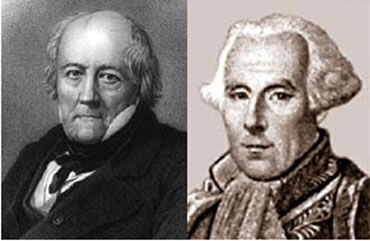
\includegraphics[width=0.99\textwidth]{./images/people/biot_and_savart.jpg}\\
     {\scriptsize
        Left: Jean Baptiste Biot (1774-1862)\\
        Right: Felix Savart (1791-1841)\\
     }
  \end{column}
  \begin{column}{0.60\textwidth}
      We seek an expression that {\bf relates steady currents (*) to constant magnetic fields.}\\
      \vspace{0.3cm}
      Such a relationship was discovered in 1820 by Biot and Savart.\\
      \vspace{0.3cm}
      It is now known as the {\bf Biot-Savart law}\\
       (pronounced: {\it bee-oh-suh-vahr}).\\
  \end{column}
\end{columns}

\vspace{0.4cm}

\noindent\rule{2cm}{0.4pt}\\
{\scriptsize
  (*) Notice that:
   \begin{itemize}
      \item There is no {\em true} steady current. It is a suitable approximation when changes are slow.
      \item A moving point charge does not constitute a steady current!
      \item A steady current {\em does not pile up}. Therefore $\partial \rho / \partial t = 0$ everywhere in space and hence,
                recalling the continuity equation, $\vec{\nabla} \vec{j} = 0$.
   \end{itemize}
}
\end{frame}

%
%
%

\begin{frame}{The Biot-Savart law}

\begin{columns}
  \begin{column}{0.40\textwidth}
     Assume a current I flowing along a conducting wire
     as shown below.\\
     \vspace{0.2cm}
     \begin{center}
       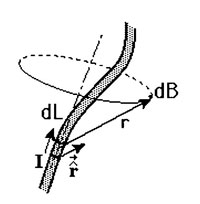
\includegraphics[width=0.99\textwidth]{./images/schematics/biot_savart.jpg}\\
      \end{center}
  \end{column}
  \begin{column}{0.60\textwidth}
     The magnetic field $d\vec{B}$ because of the current flowing through the infinitesimal
     conducting wire element $d\vec{\ell}$ is given by:
     \begin{equation*}
       d\vec{B} = \frac{\mu_0I}{4\pi} \frac{d\vec{\ell} \times \hat{r}}{r^2}
                = \frac{\mu_0I}{4\pi} \frac{d\vec{\ell} \times \vec{r}}{r^3}
     \end{equation*}
     where:
     \begin{itemize}
         \item $\vec{r}$ is the distance from $d\vec{\ell}$ to the point where we want to know the field, and\\
         \item $\mu_0$ is a constant (4$\pi\;\times\;10^{-7}$ $N/A^2$) called the {\bf permeability of free space}\\
     \end{itemize}
     \vspace{0.1cm}
     Notice the {\bf $1/r^2$ dependence} of the magnetic field (similar to the electric field).\\
  \end{column}
\end{columns}

\end{frame}

%
%
%

\begin{frame}{The Biot-Savart law}

Notice that the direction of $d\vec{B}$ is determined by the cross-product $d\vec{\ell} \times \vec{r}$.

\begin{columns}
  \begin{column}{0.50\textwidth}
     \begin{center}
        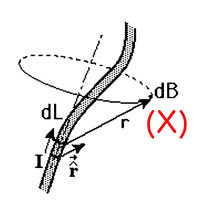
\includegraphics[width=0.60\textwidth]{./images/schematics/biot_savart_with_dB_direction.jpg}\\
      \end{center}
  \end{column}
  \begin{column}{0.50\textwidth}
     \begin{center}
        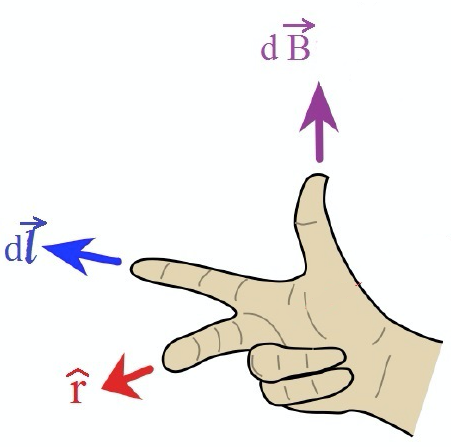
\includegraphics[width=0.60\textwidth]{./images/schematics/biot_savart_right_hand_rule.png}\\
      \end{center}
  \end{column}
\end{columns}

The {\bf superposition principle is valid for magnetostatics}.\\
The magnetic field $\vec{B}$ produced by the current flowing across the {\em entire} length L
of the conducting wire is the vector sum of the fields due to each
infinitesimal element $d\vec{\ell}$:
\begin{equation*}
       \vec{B} = \int_{L} d\vec{B} = \int_{L} \frac{\mu_0I}{4\pi} \frac{d\vec{\ell} \times \vec{r}}{r^3}
\end{equation*}

\end{frame}


%
%
%

\begin{frame}{Magnetic field around a straight wire}

\begin{columns}
  \begin{column}{0.50\textwidth}
    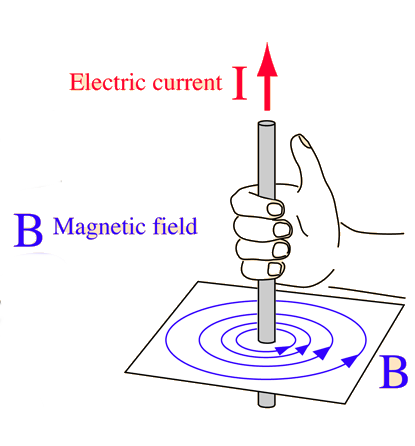
\includegraphics[width=0.98\textwidth]{./images/schematics/magnetic_field_around_wire_01.png}
  \end{column}
  \begin{column}{0.50\textwidth}
    We will use the Biot-Savart law:
    \begin{equation*}
       \vec{B} = \int_{L} \frac{\mu_0I}{4\pi} \frac{d\vec{\ell} \times \vec{r}}{r^3}
      \end{equation*}
      to calculate the magnetic field $\vec{B}$
      generated by a {\em simple} (*) current configuration:
      {\bf A single straight conducting wire}.
  \end{column}
\end{columns}

 \noindent\rule{2cm}{0.4pt}\\
 {\scriptsize
   (*) unfortunatelly, even for a simple configuration the magnetic field is not all the simple to calculate analytically.\\
 }

\end{frame}

%
%
%

\begin{frame}{Magnetic field around a straight wire}

\begin{columns}
  \begin{column}{0.40\textwidth}
    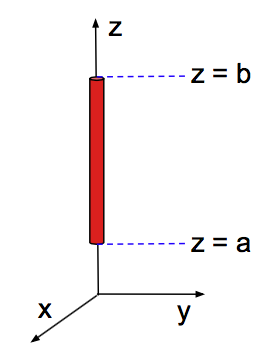
\includegraphics[width=0.98\textwidth]{./images/schematics/magnetic_field_around_wire_calc_01.png}
  \end{column}
  \begin{column}{0.60\textwidth}
  {\small
   Assume that:
   \begin{itemize}
   {\small
      \item there is current I flowing along a wire in the positive z direction, and
      \item the conductor has a finite length extending from z=a to z=b
        \begin{itemize}
        {\small
             \item later, I will consider a wire of infinite length
                       ($a \rightarrow -\infty$ and $b \rightarrow +\infty$)
        }
        \end{itemize}
   }
  \end{itemize}
  For convenience, without loss of generality,
  assume that the wire has x=0, y=0.\\
  \vspace{0.2cm}
  I will try to {\bf calculate the magnetic field at all points on the plane z=0}.
  \begin{itemize}
  {\small
      \item since, eventually, I will consider a wire with infinite length,
                this choice is as good as any.
  }
  \end{itemize}

  }
  \end{column}
\end{columns}

\end{frame}


%
%
%

\begin{frame}{Magnetic field around a straight wire}

The Biot-Savart law states that the magnetic field $\vec{B}$ at a point $\vec{r}$ is:
\begin{equation*}
  \vec{B}(\vec{r}) = \frac{\mu_0I}{4\pi} \int_{a}^{b} \frac{d\vec{\ell} \times \vec{r}}{r^3}
\end{equation*}

The element $d\vec{\ell}$ is along the positive z axis, so I can write it as:
\begin{equation*}
  d\vec{\ell} = dz \hat{z} = \Big( 0, 0, dz \Big)
\end{equation*}

The vector $\vec{r}$ points from the element $d\vec{\ell}$, which is somewhere on the z axis
(between z=a and z=b) to a point on the plane z=0. So:
\begin{equation*}
  \vec{r} = \Big( x, y, 0 \Big) - \Big( 0, 0, z \Big) = \Big( x, y, -z \Big)
\end{equation*}

The magnitude of $\vec{r}$ is:
\begin{equation*}
  r = |\vec{r}| = \Big( x^2 + y^2 + (-z)^2 \Big)^{1/2} = \Big( x^2 + y^2 + z^2 \Big)^{1/2}
\end{equation*}

\end{frame}

%
%
%

\begin{frame}{Magnetic field around a straight wire}

We can now evaluate the $d\vec{\ell} \times \vec{r}$ cross product appearing in the Biot-Savart law:\\
\begin{equation*}
  d\vec{\ell} \times \vec{r} =
   \left|
    \begin{array}{ccc}
      \hat{x} & \hat{y} & \hat{z} \\
            0 &       0 &      dz \\
            x &       y &      -z \\
    \end{array}
   \right|
   =
   \left|
    \begin{array}{cc}
            0 &  dz \\
            y &  -z \\
    \end{array}
   \right|
   \hat{x} -
   \left|
    \begin{array}{cc}
            0 &  dz \\
            x &  -z \\
    \end{array}
   \right|
   \hat{y} +
   \left|
    \begin{array}{cc}
            0 &  0 \\
            x &  y \\
    \end{array}
   \right|
   \hat{z} =
\end{equation*}

\begin{equation*}
  = \Big( -y dz \Big) \hat{x} - \Big( -x dz \Big) \hat{y} + 0 \hat{z} \Rightarrow
  d\vec{\ell} \times \vec{r} = \Big(-y, x, 0 \Big) dz
\end{equation*}

So, substituting everything back into the Biot-Savart law:
\begin{equation*}
  \vec{B}(\vec{r}) =
     \frac{\mu_0I}{4\pi} \int_{a}^{b} \frac{d\vec{\ell} \times \vec{r}}{r^3} =
     \frac{\mu_0I}{4\pi} \int_{a}^{b} \frac{\Big(-y, x, 0 \Big)}{(x^2+y^2+z^2)^{3/2}} dz
\end{equation*}

In principle we are done, but we now have to evaluate the integrals above.

\end{frame}

%
%
%

\begin{frame}{Magnetic field around a straight wire}

First, some observations. The equation:
\begin{equation*}
  \vec{B}(\vec{r}) =
     \frac{\mu_0I}{4\pi} \int_{a}^{b} \frac{\Big(-y, x, 0 \Big)}{(x^2+y^2+z^2)^{3/2}} dz
\end{equation*}

gives us all 3 components $B_{x}$, $B_{y}$ and $B_{z}$ of the $\vec{B}$ vector.
We notice that the magnetic field has no z component.
The field vectors lie on (x,y) plane with components:
\begin{equation*}
  B_{x}(\vec{r}) =
     \frac{\mu_0I}{4\pi} \int_{a}^{b} \frac{-y}{(x^2+y^2+z^2)^{3/2}} dz =
     -y \frac{\mu_0I}{4\pi} \int_{a}^{b} \frac{dz}{({\rho}^2+z^2)^{3/2}}
\end{equation*}
\begin{equation*}
  B_{y}(\vec{r}) =
     \frac{\mu_0I}{4\pi} \int_{a}^{b} \frac{x}{(x^2+y^2+z^2)^{3/2}} dz =
     x \frac{\mu_0I}{4\pi} \int_{a}^{b} \frac{dz}{({\rho}^2+z^2)^{3/2}}
\end{equation*}
where ${\rho}^2 = x^2+y^2$ is a {\em constant} for the integration over dz.

\end{frame}


%
%
%

\begin{frame}{Magnetic field around a straight wire}

Using the result we obtained for the integral $\int_{a}^{b}
\frac{dz}{({\rho}^2+z^2)^{3/2}}$ (see Optional reading),
we can now calculate the components of $\vec{B}$
\begin{equation*}
  B_{x}(\vec{r}) =
     -y \frac{\mu_0I}{4\pi} \int_{a}^{b} \frac{dz}{({\rho}^2+z^2)^{3/2}} =
     \frac{\mu_0I}{4\pi} \cdot \frac{-y}{{\rho}^{2}} \Big[ \frac{z}{({\rho}^{2}+z^{2})^{1/2}} \Big] \biggr\rvert_{z=a}^{z=b}
\end{equation*}
\begin{equation*}
  B_{y}(\vec{r}) =
     x \frac{\mu_0I}{4\pi} \int_{a}^{b} \frac{dz}{({\rho}^2+z^2)^{3/2}} =
     \frac{\mu_0I}{4\pi} \cdot \frac{x}{{\rho}^{2}} \Big[ \frac{z}{({\rho}^{2}+z^{2})^{1/2}} \Big] \biggr\rvert_{z=a}^{z=b}
\end{equation*}
and
\begin{equation*}
  B_{z}(\vec{r}) = 0
\end{equation*}

Putting it all together, we have:
\begin{equation*}
  \vec{B}(\vec{r}) = \frac{\mu_0I}{4\pi} \frac{1}{{\rho}^{2}}
    \Big[ \frac{b}{({\rho}^{2}+b^{2})^{1/2}} - \frac{a}{({\rho}^{2}+a^{2})^{1/2}}\Big] \Big( -y, x, 0 \Big)
\end{equation*}

\end{frame}

%
%
%

\begin{frame}{Magnetic field around a straight wire}

We will now obtain an approximation of the following equation
\begin{equation*}
  \vec{B}(\vec{r}) = \frac{\mu_0I}{4\pi} \frac{1}{{\rho}^{2}}
    \Big[ \frac{b}{({\rho}^{2}+b^{2})^{1/2}} - \frac{a}{({\rho}^{2}+a^{2})^{1/2}}\Big] \Big( -y, x, 0 \Big)
\end{equation*}
as $a \rightarrow -\infty$ and $b \rightarrow +\infty$.
Setting a = -b:
\begin{equation*}
  \vec{B}(\vec{r}) = \frac{\mu_0I}{4\pi} \frac{1}{{\rho}^{2}} \frac{2b}{({\rho}^{2}+b^{2})^{1/2}} \Big( -y, x, 0 \Big)
\end{equation*}
If we allow b to become infinite, then:
\begin{equation*}
\displaystyle
  \lim_{b\to\infty} \frac{2b}{({\rho}^{2}+b^{2})^{1/2}}
     \stackrel{b >> {\rho}}{\approx} \lim_{x\to\infty} \frac{2b}{(b^{2})^{1/2}} =
     \lim_{x\to\infty} \frac{2b}{b} = 2
\end{equation*}
and, therefore, the magnetic field $\vec{B}(\vec{r})$ becomes:
\begin{equation*}
  \vec{B}(\vec{r}) = \frac{\mu_0I}{2\pi {\rho}^{2}} \Big( -y, x, 0 \Big)
\end{equation*}

\end{frame}

%
%
%

\begin{frame}{Magnetic field around a straight wire}

The previous result can be rewritten as:
\begin{equation*}
  \vec{B}(\vec{r}) = \frac{\mu_0I}{2\pi {\rho}} \Big( -\frac{y}{{\rho}}, \frac{x}{{\rho}}, 0 \Big)
\end{equation*}

Let's call:
\begin{equation*}
  \hat\phi =  \Big( -\frac{y}{{\rho}}, \frac{x}{{\rho}}, 0 \Big)
\end{equation*}

It can be easily seen that $\hat\phi$ is the azimuthal unit vector:
\begin{equation*}
  \hat\phi \cdot \hat\phi = 1 \;\;\;\; and \;\;\;\; \hat{\rho} \cdot \hat\phi = 0
\end{equation*}

Our result can be summarised as:
\begin{equation*}
  \vec{B}(\vec{r}) = \frac{\mu_0I}{2\pi {\rho}} \hat\phi
\end{equation*}

\end{frame}

%
% What to remember
%

\renewcommand{\lecturesummarytitle}{Main points to remember }

\renewcommand{\summarizedlecture}{5 }

%
%
%

\begin{frame}{Lecture \summarizedlecture - \lecturesummarytitle}

\begin{itemize}

\item
An {\bf electric current is a flow of electric charge.}
It is represented by the amount of charge passing though per unit time.
\begin{equation*}
  I = \frac{dQ}{dt}
\end{equation*}
In SI, the unit of the electric current is the {\bf Ampere (A)}.

\item
The  current density $\vec{j}$ is the {\bf current per unit area  of cross-section}:
\begin{equation*}
  \vec{j} = n q \vec{u}_{d}
\end{equation*}
where n is the charge carrier density and $\vec{u}_{d}$ their average velocity.

\item
In general:
\begin{equation*}
  \vec{j} = \sigma \vec{E}
\end{equation*}
where $\sigma$ is the {\bf conductivity} of the material (SI unit: $1/(\Omega \cdot m)$).
The inverse quantity $\rho = 1/\sigma$ is called {\bf resistivity}.

\end{itemize}

\end{frame}

%
%
%
\begin{frame}{Lecture \summarizedlecture - \lecturesummarytitle (cont'd)}

\begin{itemize}

\item Magnetic and electric phenomena have a common origin.\\
          Remember the empirical evidence:
         \begin{itemize}
            \item Electric currents generate magnetic fields!
            \item Moving magnetic fields generate electric currents!
            \item There are magnetic forces between electric currents!
          \end{itemize}

\item The magnetic field (a vector field) is the magnetic effect of electric currents and magnetic materials (SI unit:  {\bf Tesla (T)})

\item The magnetic force on an electric charge q moving with velocity $\vec{u}$ in a magnetic field $\vec{B}$ is given by:
          $\vec{F} = q \vec{u} \times \vec{B}$

\item Consequently, the magnetic force on a current is
          $\vec{F} = I \int_{L} d\vec{\ell} \times \vec{B}$

\item Magnetic forces do no work on electric charges.

\item In the presence of both a magnetic field $\vec{B}$ and an electric field $\vec{E}$,
          the total (so-called Lorentz) force on charge q is:
          $\vec{F} = q \Big( \vec{E} + \vec{u} \times \vec{B} \Big)$

\end{itemize}

\end{frame}

%
%
%
\begin{frame}{Lecture \summarizedlecture - \lecturesummarytitle (cont'd)}

\begin{itemize}

\item Biot-Savart law (expresses $\vec{B}$ in terms of the current I):
     \begin{equation*}
            \vec{B} = \int_{L} d\vec{B}
                        = \frac{\mu_0I}{4\pi} \int_{L} \frac{d\vec{\ell} \times \vec{r}}{r^3}
     \end{equation*}
          where the integral is over the elements $d\vec{\ell}$ along the conductor, and $\vec{r}$
          is the distance from $d\vec{\ell}$ to the point where we want to know the field.

\vspace{0.2cm}

\item Biot-Savart in action: Magnetic field around a wire with current I:
     \begin{equation*}
           \vec{B}(\vec{r}) = \frac{\mu_0I}{2\pi \rho} \hat\phi
     \end{equation*}
         where $\rho$ is the distance from the wire and $\hat\phi$ the azimuthal unit vector.
\end{itemize}

\end{frame}


%
% Plan for the next lecture
%

\begin{frame}{At the next lecture (Lecture \nextlecture)}

We will continue studying {\bf magnetostatics}

\begin{itemize}
  \item Magnetic force between  two parallel conductors
  \item Magnetic dipole moments
  \item Principles of DC motors
  \item The curl and divergence of the magnetic field
  \item The vector potential
\end{itemize}

\end{frame}

%
% Optional reading
%




\begin{frame}[plain,c]
\begin{center}
{\Huge \bf Optional reading for Lecture \thislecture}
\end{center}
\end{frame}

%
%
%

\begin{frame}{Estimating $\int_{a}^{b} \frac{dz}{({\rho}^2+z^2)^{3/2}}$}

We can prove that:
\begin{equation*}
  \int_{a}^{b} \frac{dz}{({\rho}^2+z^2)^{3/2}} = \frac{z}{{\rho}^{2}(z^{2}+{\rho}^{2})^{1/2}} \biggr\rvert_{a}^{b}
\end{equation*}

\vspace{0.2cm}

{\small
One way to calculate this integral is to change variables ($z \rightarrow u$) and perform an integration over the variable u.
A clever variable transformation will leave us with a much simpler integral to calculate.\\

Let's try the following variable transformation:
\begin{equation*}
  z \rightarrow u = tan^{-1}\Big(\frac{z}{{\rho}})\Big)
\end{equation*}

Therefore:
\begin{equation*}
   z = {\rho} tan(u) \;\;\;\; and \;\;\;\;
  dz = {\rho} \Big( tan(u) \Big) du \Rightarrow dz = \frac{{\rho}}{cos^{2}(u)} du
\end{equation*}
}
\end{frame}

%
%
%

\begin{frame}{Estimating $\int_{a}^{b} \frac{dz}{({\rho}^2+z^2)^{3/2}}$}

{\small
With that variable transformation, the integrand becomes:
\begin{equation*}
   \frac{1}{({\rho}^2+z^2)^{3/2}} \rightarrow
     \frac{1}{({\rho}^{2}tan^{2}(u)+{\rho}^{2})^{3/2}} =
     \frac{1}{{\rho}^{3}(tan^{2}(u)+1)^{3/2}} =
     \frac{1}{{\rho}^{3}( \frac{sin^{2}(u)}{cos^{2}(u)}+1)^{3/2}} =
\end{equation*}
\begin{equation*}
   = \frac{1}{{\rho}^{3}( \frac{sin^{2}(u)+cos^{2}(u)}{cos^{2}(u)})^{3/2}} =
     \frac{1}{{\rho}^{3}( \frac{1}{cos^{2}(u)})^{3/2}} =
     \frac{cos^{3}(u)}{{\rho}^{3}}
\end{equation*}

Therefore:
\begin{equation*}
  \int_{a}^{b} \frac{dz}{({\rho}^2+z^2)^{3/2}} =
    \int_{u(a)}^{u(b)} \Big( \frac{cos^{3}(u)}{{\rho}^{3}} \Big) \Big( \frac{{\rho}}{cos^{2}(u)} du \Big) =
    \frac{1}{{\rho}^2} \int_{u(a)}^{u(b)} cos(u) du =
\end{equation*}
\begin{equation*}
   = \frac{1}{{\rho}^2} sin(u) \biggr\rvert_{u(a)}^{u(b)}
   = \frac{1}{{\rho}^2} sin\Big[ tan^{-1}\Big((\frac{z}{{\rho}})\Big) \Big]  \biggr\rvert_{a}^{b}
\end{equation*}
}
\end{frame}

%
%
%

\begin{frame}{Estimating $\int_{a}^{b} \frac{dz}{({\rho}^2+z^2)^{3/2}}$}

\begin{columns}
  \begin{column}{0.30\textwidth}
    {\small
     In order to evaluate the term
     \begin{equation*}
       sin\Big[ tan^{-1}\Big(\frac{z}{\rho}\Big) \Big] \biggr\rvert_{a}^{b}
     \end{equation*}
     appearing in the previous expression,
     consider the triangle below.\\
    }
    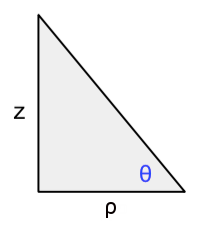
\includegraphics[width=0.85\textwidth]{./images/schematics/triangle_for_integral_in_wire_magnetic_field_calc.png}
  \end{column}
  \begin{column}{0.70\textwidth}
  {\small
    We have:
    \begin{equation*}
      tan(\theta) = \frac{z}{{\rho}} \Rightarrow
      \theta = tan^{-1}\Big( \frac{z}{{\rho}} \Big)  \Rightarrow
      sin(\theta) = sin\Big[ tan^{-1}\Big( \frac{z}{{\rho}} \Big) \Big]
    \end{equation*}
    But:
    \begin{equation*}
      sin(\theta) = \frac{z}{(z^2+{\rho}^2)^{1/2}}
    \end{equation*}
    Therefore:
    \begin{equation*}
       sin\Big[ tan^{-1}\Big( \frac{z}{{\rho}} \Big) \Big] = \frac{z}{(z^2+{\rho}^2)^{1/2}}
    \end{equation*}
    So, indeed, we showed that:
    \begin{equation*}
      \int_{a}^{b} \frac{dz}{({\rho}^2+z^2)^{3/2}} = \frac{z}{{\rho}^{2}(z^{2}+{{\rho}^{2}})^{1/2}} \biggr\rvert_{a}^{b}
    \end{equation*}
  }
  \end{column}
\end{columns}

\end{frame}


% ------------------------------------------------------------------------------
% ------------------------------------------------------------------------------
